\documentclass[a4paper,10pt]{article}
\usepackage{src/preamble}

\begin{document}

\noindent
\begin{center}
	\textbf{{\Large MAGNETI SUPERCONDUTTORI}} \\
\end{center}

\noindent
\textbf{Autore: Alessandro Biagiotti} \textit{Università degli studi di Milano, Milano, Italia}
\\

\noindent
\textbf{INTRODUZIONE:}
\\
Come già introdotto nel documento dedicato alla parte teorica, in questo secondo documento mi
dedicherò a una trattazione più pratica delle tecnologie superconduttive che sono oggi più in
utilizzo nel campo della fisica delle alte energie, e non solo (basti pensare ad applicazioni
ingegneristiche per treni ad alta velocità \cite{maglev}).

I superconduttori sono materiali caratterizzati da un brusco annullamento della resistività ($R = 0$
e non $R \approx 0$) una volta raggiunta una certa temperatura, nota come temperatura critica.
\begin{figure}[h!]
	\centering
	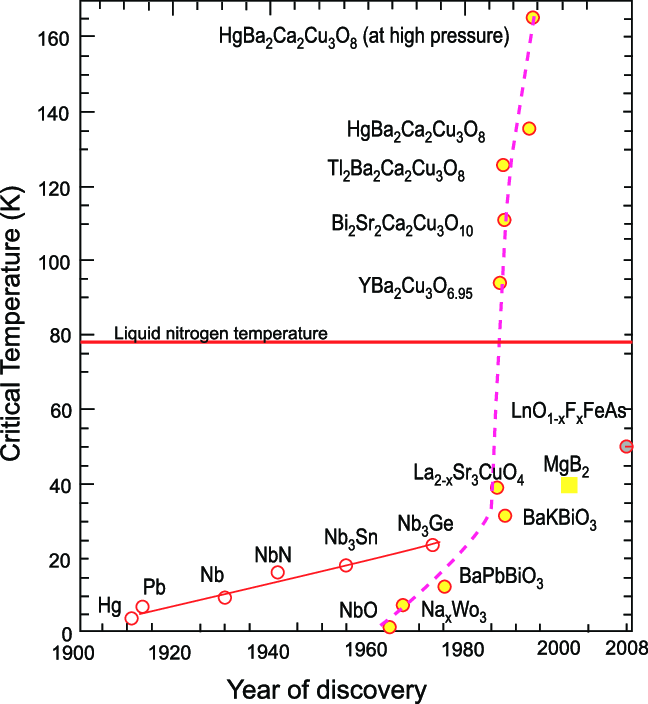
\includegraphics[scale=0.35]{fig/The-evolution-of-critical-temperatures-since-the-discovery-of-superconductivity.png}
	\caption{Temperatura critica di varie leghe che sono state scoperte nel corso degli
	anni \cite{critical-temp}}
\end{figure}
Il comportamento dei superconduttori puri è stato spiegato tramite la teoria BCS, risalente al 1957,
l'azzeramento della resistività del materiale è dovuto alla formazione delle cosiddette coppie di
Cooper.

Una coppia di Cooper è una coppia di elettroni che viaggiano insieme ed è generata da un'interazione
tra un elettrone e il reticolo cristallino (che è carico positivamente). Quest'interazione porta a
uno sbilanciamento della carica locale che passa da negativa a positiva pertanto pertanto è
possibile che un altro elettrone venga attratto da quest'assenza di carica positiva, dando vita a
una coppia di Cooper \cite{cooper-cambridge}.

In un normale conduttore la resistenza elettrica sarebbe generata dallo scattering degli elettroni
viaggianti all'interno del reticolo cristallino, all'interno di un superconduttore però la
maggioranza degli elettroni viaggiano all'interno di coppie di Cooper. Queste coppie, sebbene
interagiscano con il reticolo cristallino, non ricevono abbastanza energia per colmare l'energy gap
che le tiene insieme e, di fatto, non si dividono negli elettroni che le formano e quindi non vanno
incontro allo scattering che caratterizza la normale resistenza elettrica dei conduttori.

\bibliography{tech}

\clearpage

\end{document}
